% Options for packages loaded elsewhere
\PassOptionsToPackage{unicode}{hyperref}
\PassOptionsToPackage{hyphens}{url}
%
\documentclass[
]{article}
\usepackage{lmodern}
\usepackage{amssymb,amsmath}
\usepackage{ifxetex,ifluatex}
\ifnum 0\ifxetex 1\fi\ifluatex 1\fi=0 % if pdftex
  \usepackage[T1]{fontenc}
  \usepackage[utf8]{inputenc}
  \usepackage{textcomp} % provide euro and other symbols
\else % if luatex or xetex
  \usepackage{unicode-math}
  \defaultfontfeatures{Scale=MatchLowercase}
  \defaultfontfeatures[\rmfamily]{Ligatures=TeX,Scale=1}
\fi
% Use upquote if available, for straight quotes in verbatim environments
\IfFileExists{upquote.sty}{\usepackage{upquote}}{}
\IfFileExists{microtype.sty}{% use microtype if available
  \usepackage[]{microtype}
  \UseMicrotypeSet[protrusion]{basicmath} % disable protrusion for tt fonts
}{}
\makeatletter
\@ifundefined{KOMAClassName}{% if non-KOMA class
  \IfFileExists{parskip.sty}{%
    \usepackage{parskip}
  }{% else
    \setlength{\parindent}{0pt}
    \setlength{\parskip}{6pt plus 2pt minus 1pt}}
}{% if KOMA class
  \KOMAoptions{parskip=half}}
\makeatother
\usepackage{xcolor}
\IfFileExists{xurl.sty}{\usepackage{xurl}}{} % add URL line breaks if available
\IfFileExists{bookmark.sty}{\usepackage{bookmark}}{\usepackage{hyperref}}
\hypersetup{
  hidelinks,
  pdfcreator={LaTeX via pandoc}}
\urlstyle{same} % disable monospaced font for URLs
\usepackage{longtable,booktabs}
% Correct order of tables after \paragraph or \subparagraph
\usepackage{etoolbox}
\makeatletter
\patchcmd\longtable{\par}{\if@noskipsec\mbox{}\fi\par}{}{}
\makeatother
% Allow footnotes in longtable head/foot
\IfFileExists{footnotehyper.sty}{\usepackage{footnotehyper}}{\usepackage{footnote}}
\makesavenoteenv{longtable}
\usepackage{graphicx}
\makeatletter
\def\maxwidth{\ifdim\Gin@nat@width>\linewidth\linewidth\else\Gin@nat@width\fi}
\def\maxheight{\ifdim\Gin@nat@height>\textheight\textheight\else\Gin@nat@height\fi}
\makeatother
% Scale images if necessary, so that they will not overflow the page
% margins by default, and it is still possible to overwrite the defaults
% using explicit options in \includegraphics[width, height, ...]{}
\setkeys{Gin}{width=\maxwidth,height=\maxheight,keepaspectratio}
% Set default figure placement to htbp
\makeatletter
\def\fps@figure{htbp}
\makeatother
\setlength{\emergencystretch}{3em} % prevent overfull lines
\providecommand{\tightlist}{%
  \setlength{\itemsep}{0pt}\setlength{\parskip}{0pt}}
\setcounter{secnumdepth}{-\maxdimen} % remove section numbering

\author{}
\date{}

\begin{document}

\hypertarget{abstract}{%
\section{Abstract}\label{abstract}}

\hypertarget{introduction}{%
\section{Introduction}\label{introduction}}

\hypertarget{why-peak-load}{%
\subsection{Why peak load}\label{why-peak-load}}

The world right now requires a quick and efficient transition of most
energy usage to electric and most energy production to renewable
sources. With this changing energy paradigm will come a larger emphasis
on peak load management. Electric load growth from equipment like EV
charging and heat pumps will likely out pace distribution capacity
growth in many areas.

Public EV chargers may especially suffer from a low load factor due to
the convenience of fast charging at high power. Heat pump load factor
may be increased with architectural features such as insulation and
thermal storage, but worsening extreme weather events and challenges to
building efficiency retrofits will mean this can not be achieved
everywhere. And relative to the marginal cost of additional kWh of
energy, the marginal cost of additional kW of peak power is quite
expensive because it necessarily requires new grid infrastructure like
transformers and lines.

Distribution and transmission companies are well aware of this problem,
but infrastructure upgrades are often slowed down by regulation and
permitting. In regulatory areas where companies can own both generation
and distribution, business-as-usual grid upgrades may be prioritized
over construction of new renewable generation, which can often be
complex projects with more difficult permitting and less certain
returns. Largely due to these factors consumer prices on monthly and
annual peak load are generally increasing around the world.

\hypertarget{peak-shaving}{%
\subsection{Peak shaving}\label{peak-shaving}}

Peak load management, or peak shaving, essentially requires choosing a
power threshold and holding the load power below it. Controllable loads,
energy storage, or generation assets behind the billing meter can all be
used to reduce the load power to the threshold power. The threshold may
only apply for only certain time periods. There may be multiple
thresholds and periods each day, month, or year. There are two general
cases of peak shaving worth considering. The most generation formulation
of peak shaving control is formulated in Equation 1.

\begin{figure}
\centering
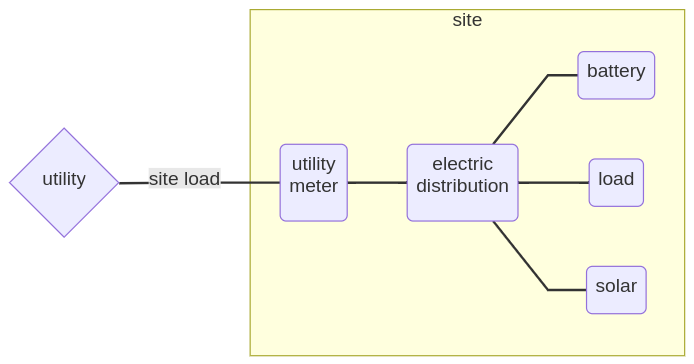
\includegraphics[width=3in,height=\textheight]{16932411489031.png}
\caption{Figure C: General schematic of case studies. The site is connected
to the electricity utility and pays for consumption according to the
electric meter. Because solar is connected behind the meter it is
directly useful for reducing the site load, and since it has a zero
marginal cost it is always dispatched at maximum available power. The
battery could be said to working on maintaining the net load below the
peak shaving threshold, where net load is load less solar.}
\end{figure}

\begin{equation}
  \begin{align}
I_{load,t} - \Sigma_i I_{gen,i,t} - \Sigma_j I_{gen\uarr,j,t} - \Sigma_k I_{load\darr,k,t} < I_{threshold,t} \\
where \\
i=generation\ asset\ with\ no\ flexibility \\
j=generation\ asset\ with\ upward\ flexibility \\
k=controllable\ load\ asset\ with\ downward\ flexibility \\
t=applicable\ timesteps\
  \end{align}
\end{equation}

Here we consider the case of no controllable load, a single battery,
solar which reduces the site load, and all values in units of average
real power over the interval \(\Delta h = 1\ hour\).

\[(2)\ P_{load,h} - P_{solar,h} - P_{batt,discharge,h} + P_{batt,charge,h}  < P_{threshold,h} \\
where \\
P_{batt,discharge,h} \ge 0 \\
P_{batt,charge,h} \le 0 \\
h \in \{0,1,2,...23\} \\\]

\hypertarget{technical-case}{%
\subsection{Technical case}\label{technical-case}}

Technical peak shaving refers to the case where a load must operate
under a technical limitation such as a maximum power agreement or
distribution transformer size. The load power must remain under the
threshold at all times, otherwise there may be a technical failure such
an activated overcurrent protection. Even if the load is technically
able to rise above the threshold, doing so may violate a contract
regarding maximum load power. The important consideration is that the
economic cost of failure to hold the load under the threshold is
prohibitively high. The time resolution of technical peak shaving
control and modeling may need to be as low as seconds or milliseconds.
Although this may be a challenging problem if the current limit is
dynamically set or if a larger network is considered, from the
perspective of dispatching the assets to shave the peak the problem is a
relatively simple one: economic dispatch such that the the load current
remains below the threshold current. Technical peak shaving might be
performed on current or apparent power rather than active power.

\begin{figure}
\centering
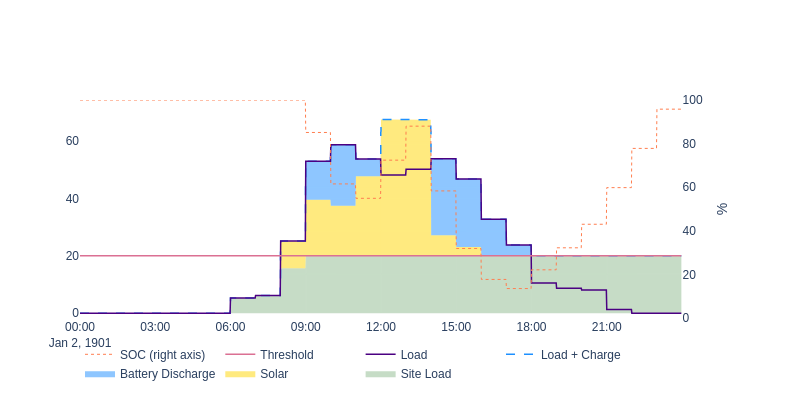
\includegraphics{/home/mjw/Insync/michael.wood@mugrid.com/Google Drive - Shared drives/Polimi/Publications/Bifacial solar and peakshaving/bifacial_peak_shaving_paper.assets/tech_shaving.png}
\caption{technical peak shaving}
\end{figure}

\emph{Figure A: The threshold is 20 kW. The battery begins the day full
at 100 kWh. By 8:00 the load has increased above the threshold to 25 kW,
but solar has also increased to 9 kW, so the site load is still below
the threshold. However at 9:00 the battery must discharge at 13 kW to
reduce to site load to 20 kW. At 12:00 the battery can recharge somewhat
due to an increase in solar and slight decrease in load. Then by 18:00
the load is less than the threshold and the battery can recharge,
increasing the site load up to the threshold.}

An example of technical peak shaving with a threshold of 20 kW is seen
in Figure A. The actual load climbs well above the threshold, but the
solar energy for that day reduces the site load considerably. Battery
discharge is required in the morning and afternoon to keep the site load
below the threshold, with some opportunistic midday charging. The
battery recharges in the evening and overnight.

\hypertarget{economic-case}{%
\subsection{Economic case}\label{economic-case}}

Rather, economic peak shaving aims to reduce what a consumer pays for
power and possibly also energy. Medium and large electric consumers
often pay a price on energy (€\(/kWh\)) and a price on power
(€\(/kWh_{peak}\)), which is often referred to as a demand charge. The
energy cost (€\(/kWh \times E_{consumed}\)) may vary with time of day,
day of week, and season of the year, which is often referred to as time
of use or peak pricing. Where there is a sufficient spread between the
peak and off-peak prices there may be the opportunity to curtail load
during high prices, use controllable loads to shift from a high price
period to a lower one, or to use energy storage to buy energy at the
lower price and reduce load during a higher price period. Instead, the
power cost (€\(/kW \times P_{max}\) ) typically applies to the max power
during the billing period, where the peak power is the average power
measured over a short interval (often 15 or 60 minutes) and only applies
to a peak period (such as )

The peak power is typically defined as the maximum load power during
certain hours of the day for a certain billing period. The peak is
calculated from a non-moving average, with a typical interval of 15
minutes or one hour.

\begin{figure}
\centering
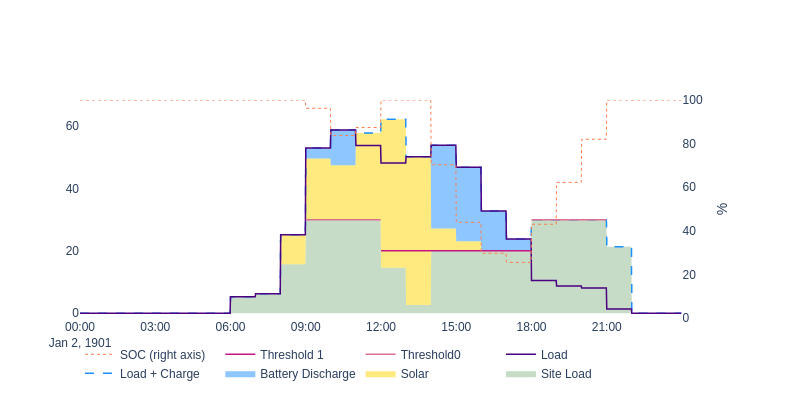
\includegraphics{/home/mjw/Insync/michael.wood@mugrid.com/Google Drive - Shared drives/Polimi/Publications/Bifacial solar and peakshaving/bifacial_peak_shaving_paper.assets/econ_shaving.png}
\caption{}
\end{figure}

\emph{Figure B: The threshold is comprised of two parts: Threshold0 at
20 kW from 12:00-18:00, and Threshold1 at 40 kW from 9:00-12:00 and
18:00-21:00. The battery begins the day full at 100 kWh. By 9:00 the
load has increased above Threshold0, solar decreases this greatly, and
the battery is discharged to further reduce the site load. However at
9:00 the battery must discharge at 13 kW to reduce to site load to 20
kW. At 11:00 and 12:00 the battery can recharge somewhat due to an
increase in solar and slight decrease in load. Then by 18:00 the load is
significantly less than the threshold and the battery can recharge,
increasing the site load up to the threshold.}

Solar contributes significantly to the load, but once the peak period
begins the battery must discharge to keep the

\begin{longtable}[]{@{}lll@{}}
\toprule
Feature & Technical Peak Shaving & Economic Peak Shaving\tabularnewline
\midrule
\endhead
Cost of violating the threshold & Prohibitively high & Depends on
tariff\tabularnewline
Averaging interval & \textless\textless{} 1 minute & 15 minutes or 1
hour (typical)\tabularnewline
Valid times of day & All & Limited (e.g. 16:00 to 21:00)\tabularnewline
Peak is reset every.. & Never & Month, year, day
(typical)\tabularnewline
\bottomrule
\end{longtable}

\hypertarget{methodology}{%
\section{Methodology}\label{methodology}}

\hypertarget{results}{%
\section{Results}\label{results}}

\hypertarget{conclusion}{%
\section{Conclusion}\label{conclusion}}

\hypertarget{bibliography}{%
\section{Bibliography}\label{bibliography}}

\end{document}
